\section{Transmisor}
\label{sec:transmisor}

\subsection{Diseño mecánico del guante}

El guante se diseñó en Solid Edge (ver sección~\ref{sec:disenio_receptor}) y se imprimió en 3D. La figura~\ref{fig:guante} muestra el conjunto. Sobre el dorso de la mano se apoya una base que aloja los cinco potenciómetros; cada dedo del operador se vincula a su potenciómetro mediante una tanza que recorre el dorso del dedo, guiada por dedales colocados en las falanges. Sobre la muñeca se ubica el soporte del ESP32.

\begin{figure}[H]
 \centering
  \subfigure[Conjunto]{
    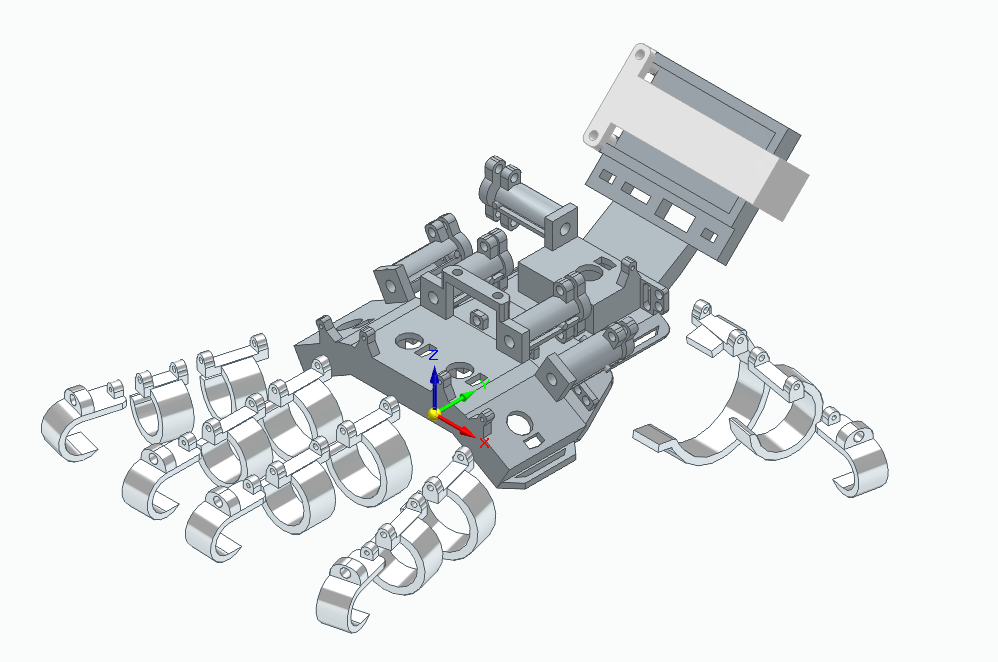
\includegraphics[width=0.48\textwidth]{Transmisor/GuanteCompleto.png}}
  \subfigure[Base dorsal]{
    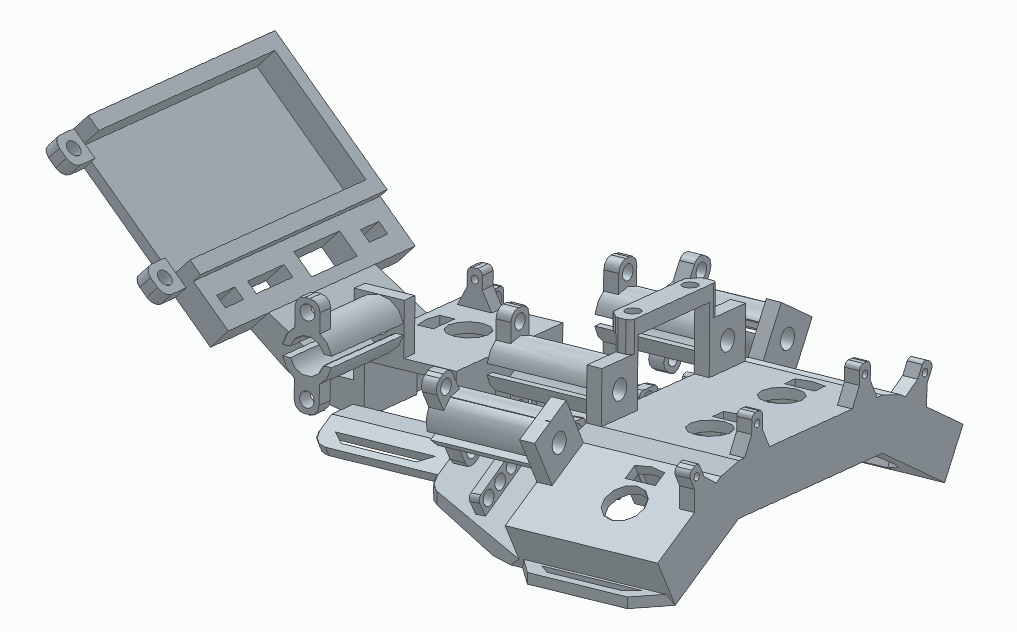
\includegraphics[width=0.45\textwidth]{Transmisor/Dorsal.png}}
 \caption{Diseño del guante transmisor.}
 \label{fig:guante}
\end{figure}

\begin{figure}[H]
 \centering
  \subfigure[Dedal de la punta]{
    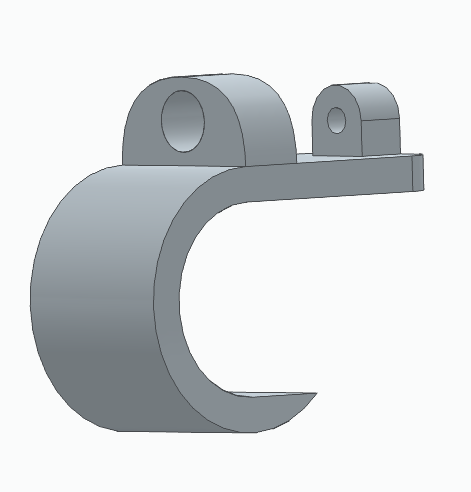
\includegraphics[width=0.18\textwidth]{Transmisor/Dedal_1.png}}
  \subfigure[Dedal guía de falange]{
    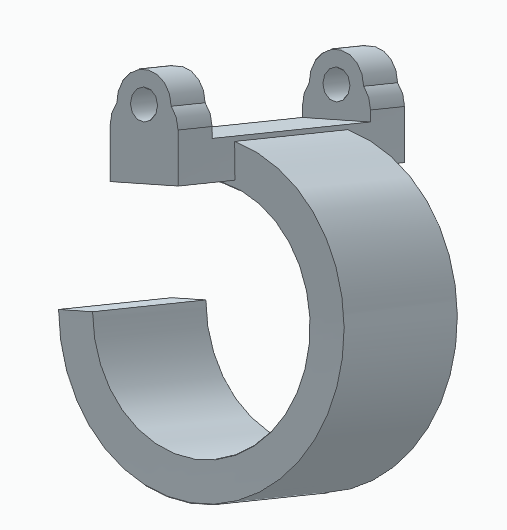
\includegraphics[width=0.18\textwidth]{Transmisor/Dedal_2.png}}
  \subfigure[Dedal del pulgar]{
    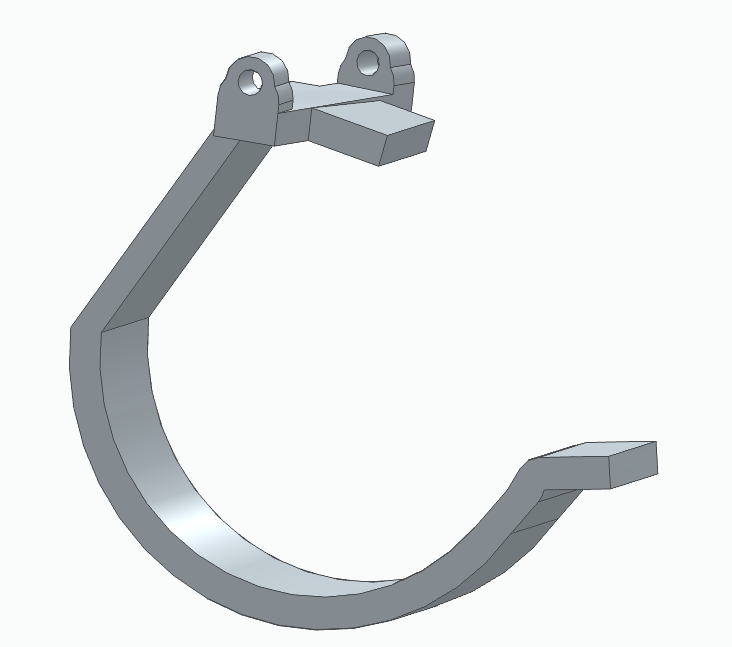
\includegraphics[width=0.18\textwidth]{Transmisor/Dedal_3_Pulgar.png}}
  \subfigure[Resortera]{
    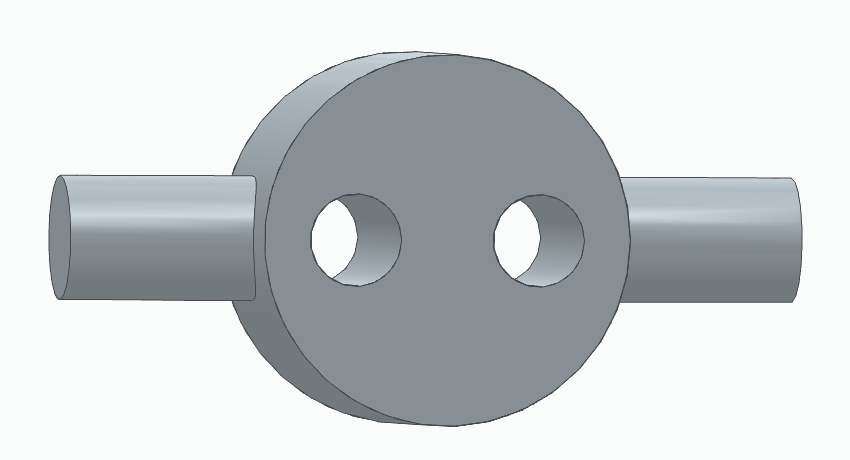
\includegraphics[width=0.2\textwidth]{Transmisor/Resortera.png}}
  \subfigure[Tapa del potenciómetro]{
    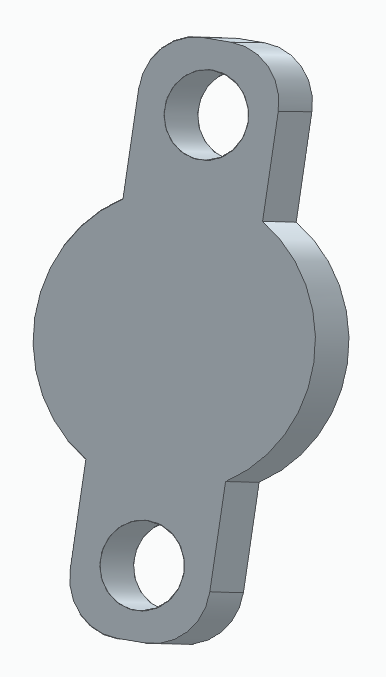
\includegraphics[width=0.1\textwidth]{Transmisor/Tapa_Pote.png}}
  \subfigure[Agarre del ESP32]{
    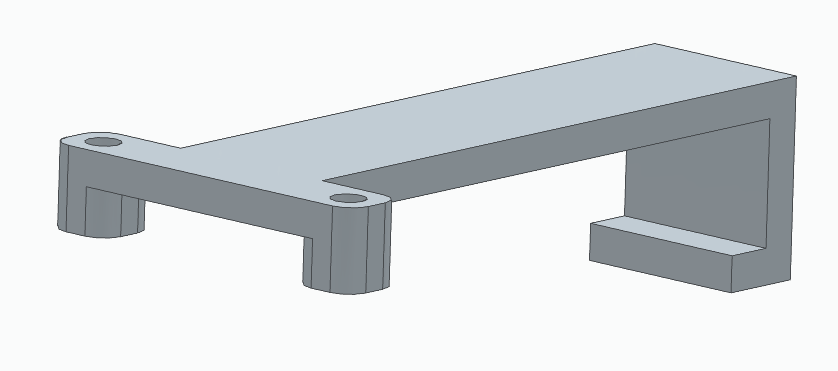
\includegraphics[width=0.25\textwidth]{Transmisor/Agarre_ESP.png}}
  \subfigure[Palanca del potenciómetro]{
    \parbox{0.2\textwidth}{\centering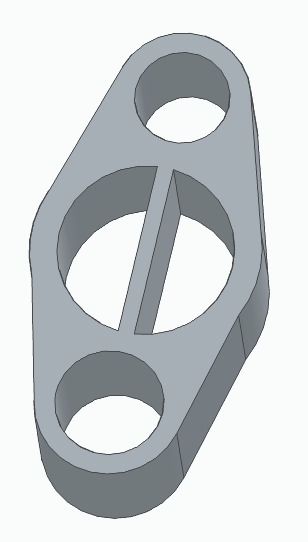
\includegraphics[width=0.08\textwidth]{Transmisor/Palanca_Pote.jpg}}}
 \caption{Piezas del guante.}
 \label{fig:piezas_guante}
\end{figure}

El movimiento de cada dedo llega a su potenciómetro a través de una tanza, siguiendo este recorrido:

\begin{enumerate}
    \item \textbf{Dedal de la punta:} un extremo de la tanza está atado a este dedal, colocado en la falange distal. Su tamaño varía ligeramente según el dedo.
    \item \textbf{Dedales guía:} la tanza recorre la parte superior del dedo sujeta a un dedal en cada falange, que la mantiene cerca del dedo. Sus medidas también dependen del dedo. En el pulgar, uno de estos dedales se ubica sobre el metacarpiano, una zona más gruesa y de forma distinta, por lo que es una pieza propia hecha más a medida.
    \item \textbf{Palanca del potenciómetro:} ya sobre el dorso de la mano, la tanza se une a una pequeña palanca impresa en 3D montada en el eje del potenciómetro (figura~\ref{fig:piezas_guante}g). Al flexionar el dedo, la tanza tira de la palanca y hace girar el eje.
    \item \textbf{Resorte y resortera:} desde la palanca, la tanza continúa hasta un pequeño tubo horizontal que contiene un resorte (hay cinco tubos sobre la base dorsal, uno por dedo), pasa por dentro del resorte y termina atada a la resortera. Al cerrar el dedo, la tanza arrastra la resortera y comprime el resorte.
    \item \textbf{Retorno:} al abrir el dedo, el resorte se descomprime, empuja la resortera hacia su posición natural y mantiene la tanza tensa, de modo que el eje del potenciómetro vuelve a la posición de reposo. El fin de ese recorrido lo marca la pieza llamada tapa del potenciómetro, que es en realidad la tapa trasera del tubo del resorte.
\end{enumerate}

El resorte cumple dos funciones: devuelve el potenciómetro a su posición cuando el dedo se abre y mantiene la tanza siempre tensa, lo que reduce la holgura al inicio del movimiento. El agarre del ESP32 fija la placa sobre la muñeca.

Al flexionar el dedo, sus tres falanges producen un desplazamiento del elemento de transmisión que, aproximadamente, es la suma de las contribuciones de cada articulación:
\begin{equation}
\Delta x \approx r_1\,\Delta\theta_1 + r_2\,\Delta\theta_2 + r_3\,\Delta\theta_3 ,
\end{equation}
donde $r_j$ es la distancia efectiva entre el elemento de transmisión y el eje de la articulación $j$. Ese desplazamiento tira de la palanca del potenciómetro, de largo $R$, y hace girar su eje un ángulo $\Delta\phi \approx \Delta x / R$. La relación es sólo aproximada: vale mientras la tanza tire casi perpendicular a la palanca, y deja de ser lineal a medida que la palanca gira. Como los radios $r_j$ dependen de la mano de cada operador y del ajuste del guante, la relación entre la flexión del dedo y la lectura del ADC no es la misma para todos los usuarios ni para todos los dedos. Además aparecen holguras al inicio del recorrido e histéresis por rozamiento. Por este motivo el firmware no usa una relación fija, sino una calibración de dos puntos por dedo (sección~\ref{sec:calibracion_dedos}). Esa calibración corrige la escala y el desplazamiento de cada dedo, pero no la falta de linealidad del mecanismo, que se traslada al ángulo del servo.

\subsection{Conexionado}

La tabla~\ref{tab:pines_tx} resume las conexiones del transmisor.

\begin{table}[H]
\centering
\begin{tabular}{l c l}
\toprule
\textbf{Señal} & \textbf{GPIO} & \textbf{Observación} \\
\midrule
Potenciómetro pulgar   & 39 & ADC1 (\texttt{SENSOR\_VN}) \\
Potenciómetro índice   & 34 & ADC1 \\
Potenciómetro medio    & 35 & ADC1 \\
Potenciómetro anular   & 32 & ADC1 \\
Potenciómetro meñique  & 33 & ADC1 \\
MPU6050 SDA            & 21 & Bus I\textsuperscript{2}C a \SI{400}{\kilo\hertz} \\
MPU6050 SCL            & 22 & Bus I\textsuperscript{2}C a \SI{400}{\kilo\hertz} \\
\bottomrule
\end{tabular}
\caption{Asignación de pines del transmisor.}
\label{tab:pines_tx}
\end{table}

Todos los potenciómetros se conectan a pines del ADC1. El ESP32 tiene dos conversores, pero el ADC2 no puede utilizarse mientras la radio Wi-Fi está activa \cite{esp32_adc}, y ESP-NOW requiere la radio encendida.

La figura~\ref{fig:conexionado_tx} muestra el conexionado completo del guante. Los cinco potenciómetros, de \SI{10}{\kilo\ohm} lineales, se conectan entre \SI{3.3}{\volt} y GND, de modo que la tensión de cada cursor nunca supera el rango de entrada del ADC. El módulo MPU6050 (GY-521) se alimenta del pin de \SI{5}{\volt} del ESP32, ya que incluye su propio regulador de \SI{3.3}{\volt}.

El guante se alimenta por el conector USB del ESP32 desde la computadora, la misma conexión que se usa para la calibración y la telemetría; el regulador de la placa genera los \SI{3.3}{\volt}. Un \textit{powerbank} de \SI{5}{\volt} queda como alternativa si se necesitara independizarlo de la computadora.

\begin{figure}[H]
    \centering
    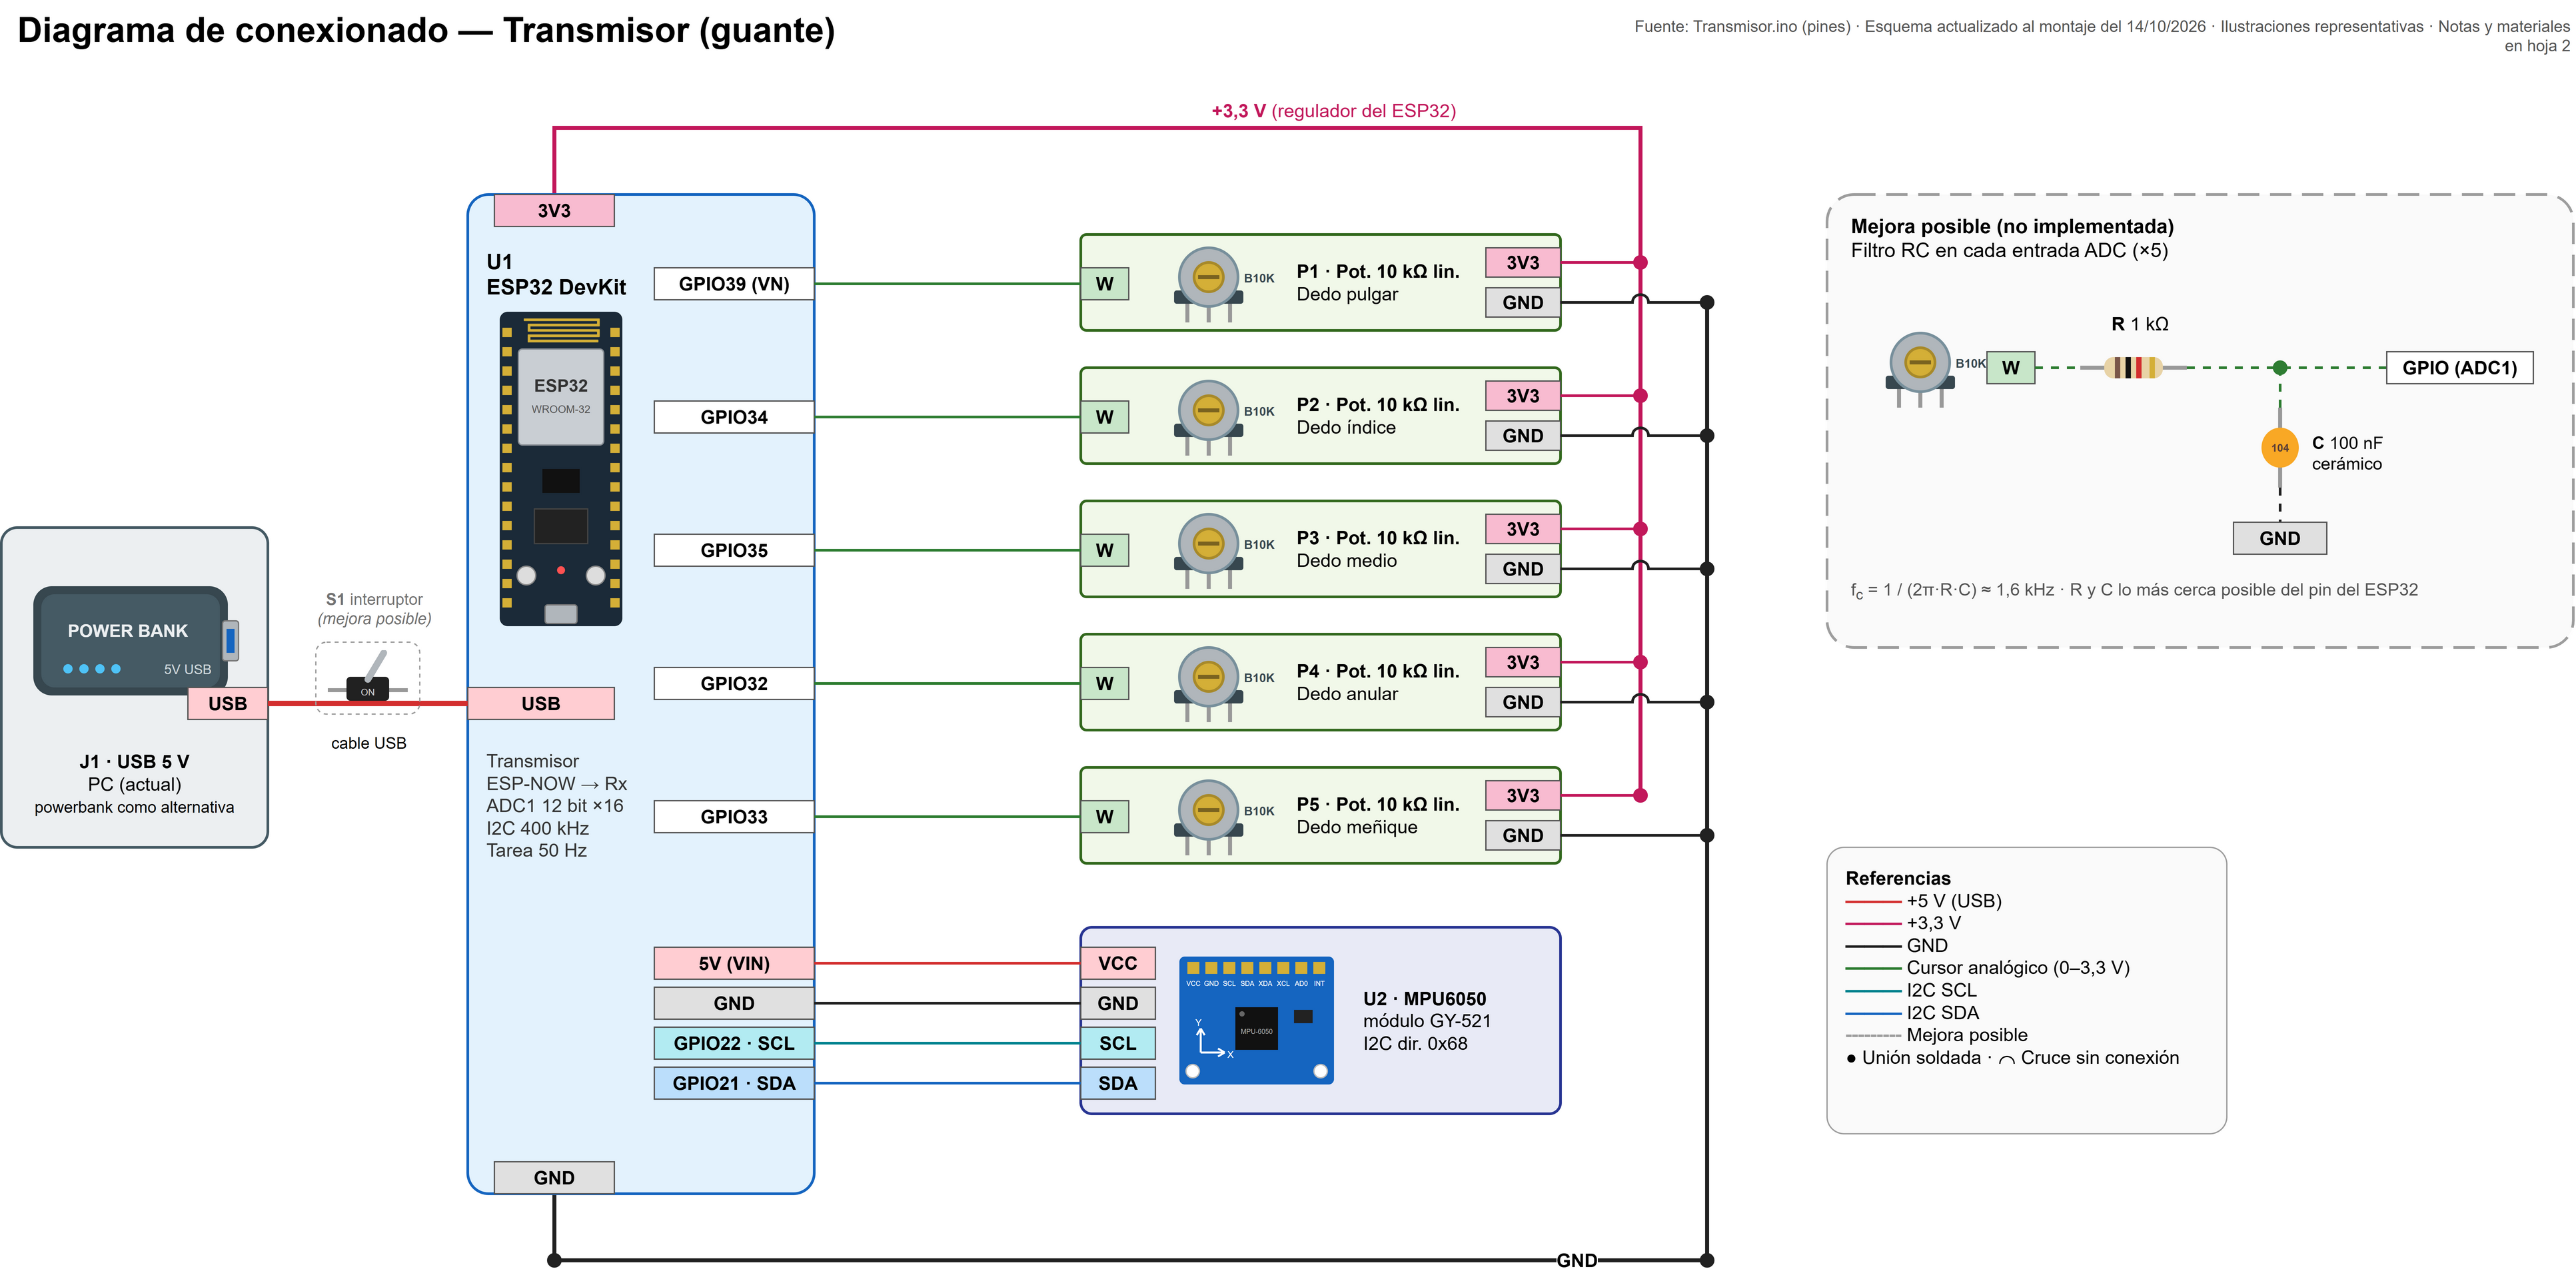
\includegraphics[width=\textwidth]{Conexionado_Transmisor_Diagrama.png}
    \caption{Diagrama de conexionado del transmisor. El filtro RC de la derecha es una mejora posible que no se implementó.}
    \label{fig:conexionado_tx}
\end{figure}

\subsection{Fundamentos de la unidad de medición inercial}

\begin{itemize}
    \item \textbf{Giróscopo:}

    Es un dispositivo que permite medir la rotación de un mecanismo. Los giróscopos de los sensores MEMS como el MPU6050 son giróscopos vibratorios de efecto Coriolis (CVG, por sus siglas en inglés). Su principio de funcionamiento es que un objeto vibratorio tiende a seguir vibrando en el mismo plano aunque su soporte rote; el efecto Coriolis hace que el objeto ejerza una fuerza sobre el soporte, y midiendo esa fuerza se determina la rotación a la que está sometido el sensor.

    \begin{figure}[H]
    \begin{center}
 		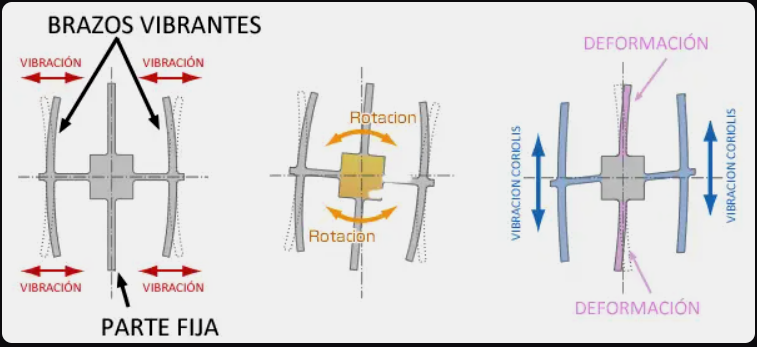
\includegraphics[scale=0.6]{Giroscopio.png}
 		\captionof{figure}{Giróscopo.}
        \label{fig:giroscopio}
    \end{center}
    \end{figure}

    Una consecuencia de emplear la fuerza de Coriolis es que estos giróscopos no registran el ángulo girado sino la \emph{velocidad angular}. Para obtener el ángulo es necesario integrar la medición respecto del tiempo. Los giróscopos responden rápido y con buena precisión en tiempos cortos, y siguen bien los cambios bruscos; pero, al integrar, cualquier error pequeño y constante en la velocidad (\textit{bias}) se acumula y el ángulo deriva (\textit{drift}). Con un \textit{bias} $b$, el error del ángulo crece linealmente con el tiempo:
    \begin{equation}
    \theta(t) = \int_0^t \omega\,dt \quad\Rightarrow\quad \theta_{\text{error}}(t) = b\,t.
    \end{equation}
    Por ejemplo, con $b = \SI{0.01}{\radian\per\second} \approx \SI{0.57}{\degree\per\second}$, que es el orden de \textit{bias} esperado para este sensor según el plan de pruebas (no un valor medido), el ángulo se desvía unos \SI{34}{\degree} en un minuto. Por eso el \textit{bias} se mide al encender y se resta (sección~\ref{sec:fusion}), y el error residual lo corrige el acelerómetro.

    \item \textbf{Acelerómetro:}

    Es un dispositivo que mide la aceleración a la que está sometido. Puede pensarse como un cuerpo sólido en cuyo interior hay una masa suspendida por resortes.

    \begin{figure}[H]
    \begin{center}
 		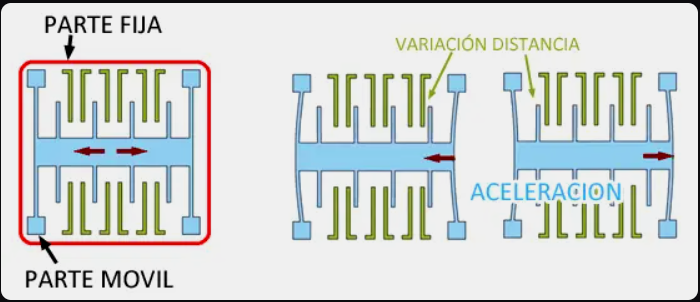
\includegraphics[scale=0.6]{Acelerometro.png}
 		\captionof{figure}{Acelerómetro.}
        \label{fig:acelerometro}
    \end{center}
    \end{figure}

    Al aplicar una aceleración al conjunto, la masa suspendida ejerce una fuerza sobre los resortes y su posición relativa dentro del sensor varía. Ese desplazamiento es proporcional a la aceleración y puede medirse. El sensor también registra la gravedad terrestre, de aproximadamente \SI{9.81}{\meter\per\second\squared}; con el sensor en reposo, la dirección de la gravedad respecto de los ejes del sensor permite determinar su orientación (figura~\ref{fig:orientacion}). La limitación es que, cuando la mano acelera, el sensor mide gravedad más movimiento y el ángulo calculado se contamina.

    \begin{figure}[H]
    \begin{center}
 		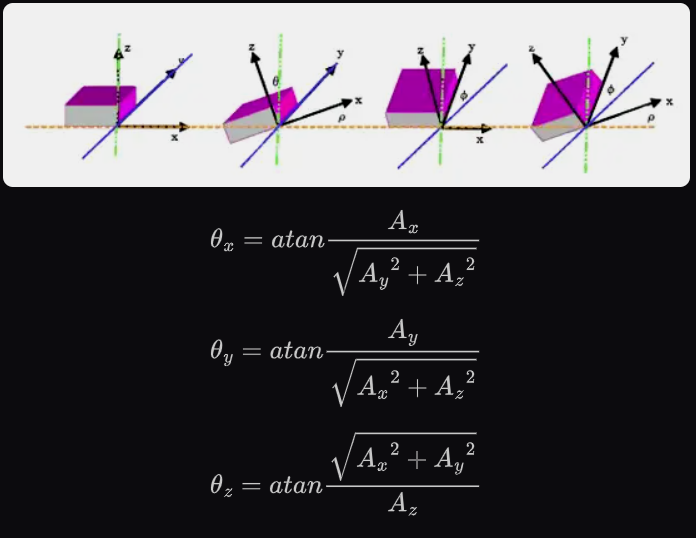
\includegraphics[scale=0.5]{Acelerometro_Calculo.png}
 		\captionof{figure}{Orientación a partir de la gravedad.}
        \label{fig:orientacion}
    \end{center}
    \end{figure}
\end{itemize}

El MPU6050 integra un acelerómetro y un giróscopo de tres ejes cada uno; es una unidad de medición inercial (IMU) de 6 grados de libertad. Cada eje entrega un valor de 16 bits, y el ESP32 lee los 14 bytes de una medición completa por I\textsuperscript{2}C. Con los rangos configurados en este proyecto, las sensibilidades de la hoja de datos son 65,5~LSB/(\si{\degree\per\second}) para el giróscopo ($\pm\SI{500}{\degree\per\second}$) y 16384~LSB/$g$ para el acelerómetro ($\pm 2\,g$). La orientación se describe con los ángulos de Tait-Bryan: rotaciones en torno al eje X (\textit{roll}), al eje Y (\textit{pitch}) y al eje Z (\textit{yaw}) (figura~\ref{fig:rotaciones}). En este proyecto se utilizan el \textit{pitch}, que corresponde a la flexión de la muñeca hacia arriba y abajo, y el \textit{roll}, que corresponde a la rotación de la mano. El \textit{yaw} no puede obtenerse del acelerómetro (la gravedad no cambia al girar alrededor del eje vertical) y no se utiliza.

\begin{figure}[H]
    \begin{center}
 		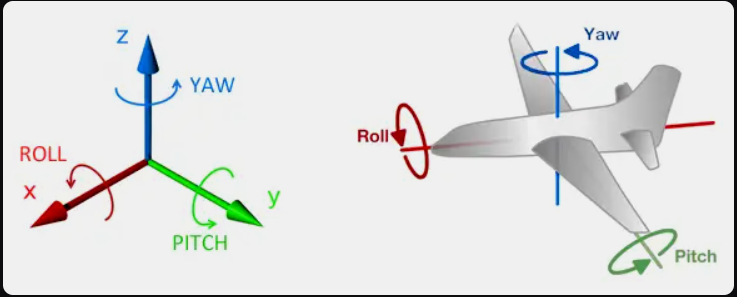
\includegraphics[scale=0.5]{Rotaciones.png}
 		\captionof{figure}{Rotaciones de Tait-Bryan.}
        \label{fig:rotaciones}
    \end{center}
\end{figure}

Las dos fuentes de información son complementarias: el giróscopo es confiable a corto plazo y el acelerómetro a largo plazo. Para aprovechar ambas se las combina con un filtro de fusión, que se describe en la sección~\ref{sec:fusion}.

\subsection{Firmware del transmisor}

\subsubsection{Inicialización}

Al encender, la función \texttt{setup()} ejecuta los siguientes pasos:

\begin{enumerate}
    \item Configura el ADC con 12 bits de resolución (0 a 4095) y atenuación de \SI{11}{\deci\bel}, que amplía el rango de entrada a aproximadamente 0--\SI{3.3}{\volt}.
    \item Carga la calibración de los dedos desde la memoria no volátil (sección~\ref{sec:calibracion_dedos}).
    \item Libera el bus I\textsuperscript{2}C (ver más abajo) e inicia la comunicación con el MPU6050 a \SI{400}{\kilo\hertz}, con hasta cinco intentos.
    \item Configura el MPU6050: acelerómetro en $\pm 2\,g$ (máxima resolución; la mano no supera esa aceleración en uso normal), giróscopo en $\pm\SI{500}{\degree\per\second}$ y filtro pasa-bajos interno en \SI{44}{\hertz}. Luego calibra el sensor en reposo (sección~\ref{sec:fusion}).
    \item Inicia la radio en modo estación, desactiva el ahorro de energía de la radio (\texttt{WiFi.setSleep(false)}), que agrega latencia, y registra al receptor como destino (\textit{peer}) de ESP-NOW mediante su dirección MAC, sin cifrado.
    \item Crea la tarea periódica \texttt{tareaTransmision} en el núcleo 1.
\end{enumerate}

\paragraph{Recuperación del bus I\textsuperscript{2}C.} Si el ESP32 se reinicia en medio de una lectura, el MPU6050 puede quedar a mitad de la transmisión de un byte, manteniendo la línea SDA en nivel bajo. El bus queda bloqueado y la inicialización falla aunque el sensor funcione. Para evitarlo, antes de iniciar el bus se generan manualmente nueve pulsos de reloj en SCL, suficientes para que el esclavo termine de enviar el byte pendiente y libere SDA, seguidos de una condición de STOP. Es el procedimiento de \textit{bus clear} de la especificación de I\textsuperscript{2}C \cite{nxp_i2c}.

\subsubsection{Ciclo periódico}

La tarea \texttt{tareaTransmision} se ejecuta cada \SI{20}{\milli\second} (\SI{50}{\hertz}) mediante \texttt{vTaskDelayUntil()}, que mide el período desde el despertar anterior y no desde el final del trabajo \cite{freertos}. A diferencia de un \texttt{delay(20)} al final del bucle, el período no se alarga con el tiempo de cómputo: la tarea despierta en instantes absolutos (0, 20, \SI{40}{\milli\second}, etc.). Si un ciclo excediera los \SI{20}{\milli\second}, \texttt{vTaskDelayUntil()} no esperaría y el ciclo siguiente arrancaría enseguida, de modo que la grilla de tiempos se mantiene y el atraso no se acumula. La figura~\ref{fig:ciclo_tx} muestra el orden de cada ciclo.

\begin{figure}[H]
\centering
\begin{tikzpicture}[node distance=0.45cm, every node/.style={font=\small}]
  \node[bloque, fill=gray!10] (t) {Despertar (cada \SI{20}{\milli\second})};
  \node[bloque, below=of t] (imu) {Leer MPU6050 y aplicar el filtro complementario\\Calcular ángulos de servo de la muñeca};
  \node[draw, diamond, aspect=2.5, below=of imu, inner sep=1pt, fill=yellow!10] (cal) {¿Calibrando?};
  \node[bloque, below=of cal] (ded) {Leer los 5 potenciómetros (16 muestras c/u)\\Convertir a ángulo con la calibración};
  \node[bloque, below=of ded] (env) {Armar paquete, secuencia y checksum\\Enviar por ESP-NOW};
  \node[bloque, below=of env] (tel) {Telemetría serie (1 de cada 10 ciclos)};
  \draw[flecha] (t) -- (imu);
  \draw[flecha] (imu) -- (cal);
  \draw[flecha] (cal) -- node[right]{No} (ded);
  \draw[flecha] (ded) -- (env);
  \draw[flecha] (env) -- (tel);
  \draw[flecha] (cal.east) -- node[above]{Sí} ++(2.8,0) |- (t.east);
  \draw[flecha] (tel.west) -- ++(-3.8,0) |- (t.west);
\end{tikzpicture}
\caption{Ciclo de la tarea de transmisión.}
\label{fig:ciclo_tx}
\end{figure}

\subsubsection{Sensado de los dedos}

\paragraph{Sobremuestreo.} El ADC del ESP32 presenta ruido de varias cuentas. Para reducirlo, cada lectura es el promedio de 16 conversiones separadas por \SI{50}{\micro\second}. Si el ruido es aleatorio e independiente entre muestras, el promedio de $N$ muestras reduce su desviación estándar en un factor $\sqrt{N}$:
\begin{equation}
\sigma_{\bar{x}} = \frac{\sigma}{\sqrt{N}} = \frac{\sigma}{4} \quad (N = 16).
\end{equation}
El promedio no corrige la alinealidad propia del ADC; ésta queda absorbida en parte por la calibración de dos puntos. Leer los cinco dedos de esta forma insume del orden de \SI{5}{\milli\second}, que entra con holgura en el período de \SI{20}{\milli\second}.

\paragraph{Calibración de dos puntos.}
\label{sec:calibracion_dedos}
Cada dedo tiene dos valores de calibración: la lectura con la mano abierta, $ADC_{\min}$, y con el puño cerrado, $ADC_{\max}$. Se almacenan en la memoria flash no volátil (NVS) del ESP32 mediante la librería \texttt{Preferences}, por lo que se conservan al apagar y al reprogramar el firmware. Si nunca se calibró, se usan 1200 y 3200 por defecto. La lectura se convierte a un ángulo lógico del dedo, entre \SI{25}{\degree} (extendido) y \SI{90}{\degree} (flexionado), por interpolación lineal y saturación:
\begin{equation}
\theta_{\text{dedo}} = \operatorname{sat}_{[25,\,90]}\!\left( 25 + \left(ADC - ADC_{\min}\right)\frac{90 - 25}{ADC_{\max} - ADC_{\min}} \right).
\end{equation}
La saturación evita que, si el operador abre o cierra la mano más que durante la calibración, el ángulo salga del rango mecánico de la mano robótica. Como la fórmula admite $ADC_{\max} < ADC_{\min}$, un potenciómetro montado al revés también funciona sin cambios en el código.

\paragraph{Procedimiento de calibración.} Se inicia enviando el carácter \texttt{c} por el monitor serie. El firmware pide abrir la mano y presionar ENTER (registra los mínimos promediando 32 muestras), luego cerrar el puño y presionar ENTER (registra los máximos) y finalmente guarda los diez valores en la NVS. Durante la calibración la tarea de transmisión deja de leer los dedos, de transmitir y de imprimir telemetría; sólo sigue leyendo la IMU para no perder el estado del filtro de la muñeca. En consecuencia, el receptor deja de recibir paquetes, entra en su modo de seguridad y lleva la mano a la posición de reposo (sección~\ref{sec:fsm}); al terminar la calibración el envío se reanuda y la mano vuelve a seguir al guante sin intervención. Este comportamiento se agregó en la versión 2.3.0 y se verificó en hardware.

\subsubsection{Estimación de la orientación de la muñeca}
\label{sec:fusion}

\paragraph{Calibración en reposo.} Al encender, con la mano quieta, se toman 500 lecturas (aproximadamente \SI{1.5}{\second}) y se calculan:
\begin{itemize}
    \item el \textit{bias} de los ejes X e Y del giróscopo, es decir, el valor que miden estando quietos, que luego se resta en cada lectura; y
    \item los ángulos iniciales de \textit{pitch} y \textit{roll} según el acelerómetro, para que el filtro arranque en la orientación real y no en \SI{0}{\degree}.
\end{itemize}

\paragraph{Ángulos por acelerómetro.} Con el sensor en reposo, la inclinación se obtiene de las componentes de la gravedad \cite{pedley_an3461}:
\begin{equation}
\phi_{acc} = \operatorname{atan2}\left(a_y,\ a_z\right), \qquad
\theta_{acc} = \operatorname{atan2}\left(-a_x,\ \sqrt{a_y^2 + a_z^2}\right),
\label{eq:angulos_acc}
\end{equation}
donde $\phi$ es el \textit{roll} y $\theta$ el \textit{pitch}. Al ser cocientes, el resultado no depende de que la aceleración esté expresada en \si{\meter\per\second\squared} o en unidades de $g$.

\paragraph{Filtro complementario.} Para cada ángulo se combina la integración del giróscopo con el ángulo del acelerómetro \cite{colton2007, mahony2008}:
\begin{equation}
\theta_k = \alpha\left(\theta_{k-1} + \omega_k\,\Delta t\right) + (1-\alpha)\,\theta_{acc,k}, \qquad \alpha = 0{,}98,
\label{eq:complementario}
\end{equation}
donde $\omega_k$ es la velocidad angular medida, sin \textit{bias}, y $\Delta t$ el tiempo transcurrido desde la lectura anterior, medido con \texttt{micros()} (si resultara nulo o mayor a \SI{100}{\milli\second}, se usa \SI{20}{\milli\second}).

\paragraph{Por qué se llama complementario.} La ecuación~\eqref{eq:complementario} admite dos lecturas. Tomada tal como está escrita, con las entradas $\theta_{acc}$ y $\omega_k\,\Delta t$ (el giro medido en cada ciclo), su transformada Z es
\begin{equation}
\Theta(z) = \underbrace{\frac{1-\alpha}{1-\alpha z^{-1}}}_{H_{acc}(z)}\,\Theta_{acc}(z) + \frac{\alpha}{1-\alpha z^{-1}}\,\Delta t\,\Omega(z).
\label{eq:complementario_directa}
\end{equation}
Los dos canales son pasa-bajos con el mismo polo en $z = \alpha$, con ganancia en continua 1 para el acelerómetro y $\alpha/(1-\alpha) = 49$ para $\omega\,\Delta t$. Vista así, la ecuación no contiene ningún pasa-altos: sólo suaviza las dos entradas, y lo que suma uno son los pesos $\alpha$ y $1-\alpha$, no las transferencias.

El nombre aparece al tomar como entrada del giróscopo el ángulo que daría por sí solo, es decir, la suma de todos sus giros: $\theta_{g,k} = \theta_{g,k-1} + \omega_k\,\Delta t$. Como entonces $\Delta t\,\Omega(z) = (1-z^{-1})\,\Theta_g(z)$, reemplazando en~\eqref{eq:complementario_directa} queda
\begin{equation}
\Theta(z) = H_{acc}(z)\,\Theta_{acc}(z) + H_g(z)\,\Theta_g(z), \qquad
H_g(z) = \frac{\alpha\,(1-z^{-1})}{1-\alpha z^{-1}}, \qquad
H_{acc}(z) + H_g(z) = 1 .
\end{equation}
Respecto de $\theta_g$, el canal del giróscopo es un pasa-altos: ganancia nula en continua y cercana a uno en las frecuencias altas. Como $\theta_g$ y $\theta_{acc}$ estiman el mismo ángulo y las dos transferencias suman uno en todas las frecuencias, el filtro toma los cambios rápidos del giróscopo y el valor de fondo del acelerómetro, y lo que uno descarta lo aporta el otro; de ahí el nombre de \emph{complementario}. El firmware nunca calcula $\theta_g$ por separado: el pasa-altos queda implícito en la ecuación~\eqref{eq:complementario}. La constante de tiempo que separa ambas regiones es
\begin{equation}
\tau = \frac{\alpha\,\Delta t}{1-\alpha} = \frac{0{,}98 \times \SI{0.02}{\second}}{0{,}02} \approx \SI{0.98}{\second}.
\end{equation}
Para movimientos más rápidos que $\tau$ domina el giróscopo, que responde sin retardo; para tiempos mayores domina el acelerómetro, que corrige lentamente la deriva.

La ganancia de 49 del canal $\omega\,\Delta t$ tiene una consecuencia práctica. Con un \textit{bias} residual $b$, el ángulo ya no deriva sin límite como en el giróscopo solo, sino que queda desplazado un valor fijo:
\begin{equation}
\Delta\theta = \frac{\alpha}{1-\alpha}\,b\,\Delta t = \tau\, b .
\end{equation}
Con el \textit{bias} de \SI{0.57}{\degree\per\second} usado como ejemplo al describir el giróscopo, que sin el filtro haría derivar el ángulo unos \SI{34}{\degree} por minuto, el error sería de unos \SI{0.56}{\degree}. Por eso igual conviene medir y restar el \textit{bias} al encender. La velocidad angular se integra con el signo que hace que un giro positivo aumente el mismo ángulo que calcula~\eqref{eq:angulos_acc}: $+\omega_y$ aumenta el \textit{pitch} y $+\omega_x$ aumenta el \textit{roll}.

\begin{lstlisting}[caption={Filtro complementario en la tarea de transmisión.}, label={cod:complementario}]
float gyroRatePitch = (g.gyro.y - gyroBiasY) * RAD_TO_DEG;
float gyroRateRoll  = (g.gyro.x - gyroBiasX) * RAD_TO_DEG;

anguloPitch = ALPHA_COMPLEMENTARIO * (anguloPitch + gyroRatePitch * dt)
            + (1.0f - ALPHA_COMPLEMENTARIO) * pitchAcc(a);

// Cerca de ±90° de pitch el roll del acelerómetro es indeterminado
// (gimbal lock), así que dejamos el último valor bueno
if (fabs(anguloPitch) < 80.0f) {
    anguloRoll = ALPHA_COMPLEMENTARIO * (anguloRoll + gyroRateRoll * dt)
               + (1.0f - ALPHA_COMPLEMENTARIO) * rollAcc(a);
}
\end{lstlisting}

\paragraph{Singularidad del \textit{roll}.} Cuando el \textit{pitch} se acerca a $\pm\SI{90}{\degree}$ (mano apuntando hacia arriba o hacia abajo), $a_y$ y $a_z$ tienden a cero y $\operatorname{atan2}(a_y, a_z)$ queda indeterminado. Por eso, si $|\theta| \geq \SI{80}{\degree}$, el \textit{roll} no se actualiza y conserva su último valor válido. Es la manifestación práctica del bloqueo de cardán (\textit{gimbal lock}) de los ángulos de Euler.

\paragraph{Filtro interno del MPU6050.} El sensor incluye un filtro pasa-bajos digital (DLPF) configurable que atenúa las vibraciones a costa de un retardo \cite{mpu6050_regmap}. Se eligió el ajuste de \SI{44}{\hertz}, que reduce el retardo en unos \SI{3.5}{\milli\second} respecto del de \SI{21}{\hertz} utilizado en versiones anteriores; el ruido adicional lo absorbe el filtro complementario.

\begin{table}[H]
\centering
\begin{tabular}{c c c}
\toprule
\textbf{Ajuste DLPF} & \textbf{Retardo acelerómetro} & \textbf{Retardo giróscopo} \\
\midrule
\SI{21}{\hertz} (versiones 2.0.0 y 2.1.0) & \SI{8.5}{\milli\second} & \SI{8.3}{\milli\second} \\
\textbf{\SI{44}{\hertz} (desde la versión 2.2.0)} & \textbf{\SI{4.9}{\milli\second}} & \textbf{\SI{4.8}{\milli\second}} \\
\bottomrule
\end{tabular}
\caption{Retardo del filtro interno del MPU6050 según el mapa de registros del fabricante.}
\label{tab:dlpf}
\end{table}

\subsubsection{Conversión a ángulos de servo}
\label{sec:mapeo_munieca}

Antes de convertir, a cada ángulo se le resta una constante de ajuste de montaje, igual al ángulo que mide el sensor con la mano en la pose neutra (en el código, \texttt{TRIM\_PITCH\_DEG} y \texttt{TRIM\_ROLL\_DEG}). El \textit{pitch} se convierte con dos tramos lineales que comparten el punto neutro (mano horizontal, servo en \SI{57}{\degree}), porque el rango útil de la muñeca del operador (\SI{45}{\degree} hacia arriba y \SI{25}{\degree} hacia abajo) y el del servo alrededor de su neutro (\SI{32}{\degree} y \SI{33}{\degree}) no son simétricos:
\begin{equation}
\theta_{servo,V} =
\begin{cases}
57 - \dfrac{p}{45}\,(57 - 25) & \text{si } p \geq 0 \\[2ex]
57 + \dfrac{p}{-25}\,(90 - 57) & \text{si } p < 0
\end{cases}
\end{equation}
donde $p = \operatorname{sat}_{[-25,\,45]}\left(\theta - \theta_{trim}\right)$ es el \textit{pitch} corregido y saturado al rango útil.
La rotación se convierte de forma lineal, de modo que la mano plana corresponde al servo centrado:
\begin{equation}
\theta_{servo,R} = \operatorname{sat}_{[0,\,180]}\left(\phi - \phi_{trim} + 90\right), \qquad \phi - \phi_{trim} \in [-90, 90].
\end{equation}
Los cálculos se hacen en punto flotante y el resultado se redondea al grado más cercano antes de empaquetarlo.

\subsubsection{Empaquetado y envío}

En cada ciclo se completa la estructura del paquete con la firma, el número de secuencia y la suma de verificación (sección~\ref{sec:protocolo}) y se envía con \texttt{esp\_now\_send()} en modo \textit{unicast}. En este modo, la radio del receptor responde con un acuse de recibo (ACK) a nivel MAC y, si no llega, la radio reintenta automáticamente. El resultado se informa en el callback \texttt{OnDataSent()} y se muestra en la telemetría serie como \texttt{OK} o \texttt{NO\_ACK}. La telemetría se imprime sólo uno de cada diez ciclos (\SI{5}{\hertz}), porque escribir en el puerto serie es lento y a \SI{50}{\hertz} afectaría la temporización.
